
\chapter{Background}
Artificial Intelligence has advanced at a remarkable rate recently, with Deep Learning models achieving state-of-the-art performance in various tasks. These models, which include Transformers, Convolutional Neural Networks (CNNs), and Generative Pretrained Transformers (GPTs), have been applied to a wide range of applications, including Natural Language Processing (NLP) and Computer Vision. This chapter provides an overview of the critical concepts and architectures underpinning these models and their applications in the on-site insect detection and classification system. The chapter also discusses prompt engineering, a technique used to optimize the performance of language models like GPT.

\section{Transformers}
Transformers are a type of Deep Learning Neural Network architecture \cite{transformers_1}. They have become the foundation for many state-of-the-art NLP and Computer Vision models. The primary value of the new transformer architecture is its ``self-attention mechanism," which enables selection across multiple inputs based on importance when processing each element. This mechanism enables transformers to effectively capture long-range dependencies and relationships in the input data.

Transformers have been widely used for machine translation, language modeling, and text classification. The Transformer architecture has an encoder and decoder component, each composed of multiple layers of self-attention and feedforward neural networks. The encoder takes in the input sequence for processing, and the decoder creates the output sequence. The generic model architecture of a Transformer developed by Google is shown in Fig \ref{fig:3.1}.

\begin{figure}[H]
\begin{center}
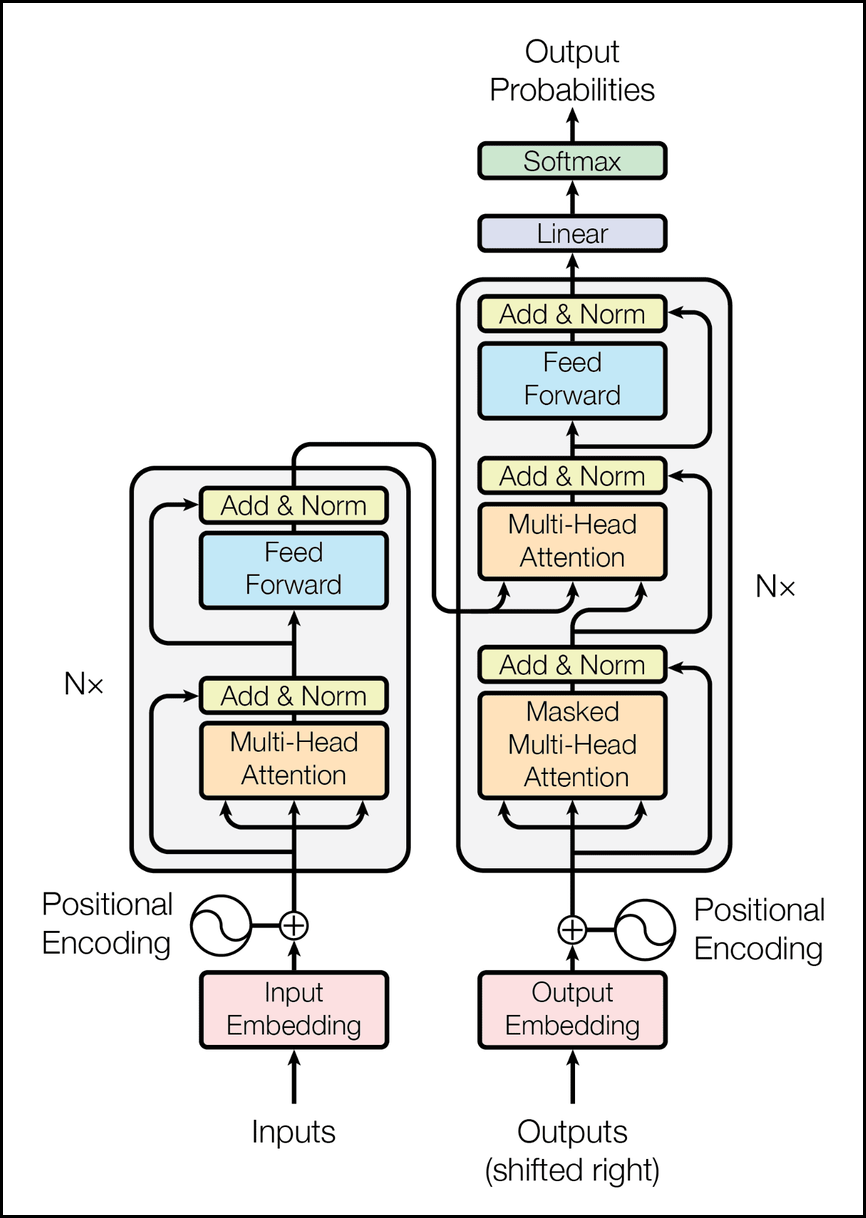
\includegraphics[width=0.85\linewidth]{Honors_Thesis/Figures/3.1.png}
\end{center}
\caption{The Transformer - model architecture \cite{transformers_1}.}
\label{fig:3.1}
\end{figure}

\section{Computer Vision Model}
The on-site insect detection and classification system leverages the power of deep learning models to achieve accurate and efficient results. By building upon previous research in the field of Computer Vision, the system employs a combination of detection and classification models to identify and categorize insects in images captured by the camera. The use of transformers in the computer vision domain allows the system to capture complex patterns and relationships in the image data, leading to high levels of accuracy and reliability. The following sections cover the details of the deep learning models and techniques used in the system.

\subsection{Deep Learning}
Within the field of Machine Learning exists its subset, Deep Learning, which involves the training of Neural Networks with many layers to perform tasks such as image and speech recognition \cite{lecun_bengio_hinton_2015}. A specific type of Deep Learning model used in Computer Vision is Convolutional Neural Networks (CNNs). CNNs consist of convolutional layers that automatically learn spatial rankings of features from the input data.

The ImageNet classification challenge has been a driving force behind developing Deep Learning models for Computer Vision. Notably, the AlexNet architecture \cite{NIPS2012_c399862d} achieved a breakthrough in the ImageNet challenge using deep CNNs. YOLO (You Only Look Once) is another popular deep learning model for real-time object detection and classification \cite{redmon2016}. What makes YOLO more efficient than traditional methods is its ability to process the entire inputted image in one go rather than multiple possessions. YOLO employs a single CNN that divides the input image into a grid and predicts each grid cell's bounding boxes and class probabilities. The model then thresholds these predictions to produce the final object detections.

Vision transformers \cite{DBLP:journals/corr/abs-2010-11929} are a recent development that applies transformer architecture to computer vision tasks. They divide an image into fixed-size patches and process them as a sequence using self-attention mechanisms. The model architecture of a Vision Transformer developed by Google is shown in Fig \ref{fig:3.2}.

\begin{figure}[H]
\begin{center}
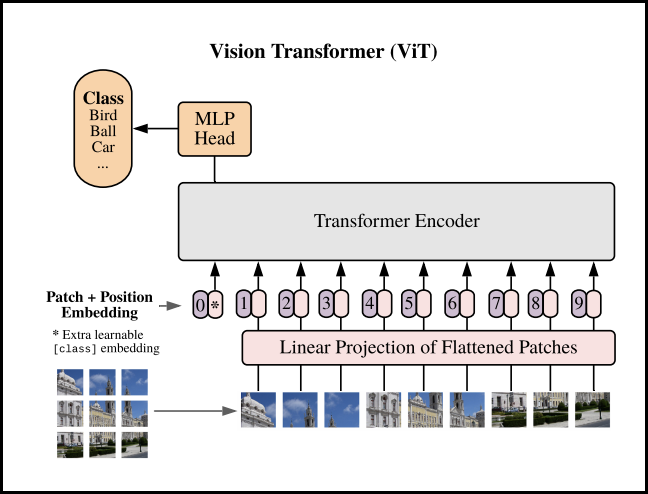
\includegraphics[width=0.7\linewidth]{Honors_Thesis/Figures/3.2.png}
\end{center}
\caption{The Vision Transformer - model architecture \cite{DBLP:journals/corr/abs-2010-11929}.}
\label{fig:3.2}
\end{figure}

\subsection{Insect Detection and Classification Models}
The on-site system that is responsible for sending insect data and running the Machine Learning models uses advanced AI detection and classification models to locate objects in the image returned from the camera and assign classes to those detections based on an insect dataset \cite{helton_luu_dowling_2022}.

The dataset used combines manually sourced images of bee flies, the IP102 dataset \cite{8954351}, and the EU Moths dataset \cite{DBLP:conf/gi/KorschBD21}. The 2,205 image dataset was manually annotated for the detection model to work. The final detection model was implemented using a Detection Transformer (DETR) as opposed to yolov5 due to its higher accuracy \cite{li2022dndetr}. Similarly, the final classification model was implemented using a Vision Transformer instead of a CNN to improve accuracy in recognizing minuscule differences between insect specifies. Using both models, the automated system can produce annotated images and extract data from them, as shown in Fig \ref{fig:3.3}.

\begin{figure}[H]
\begin{center}
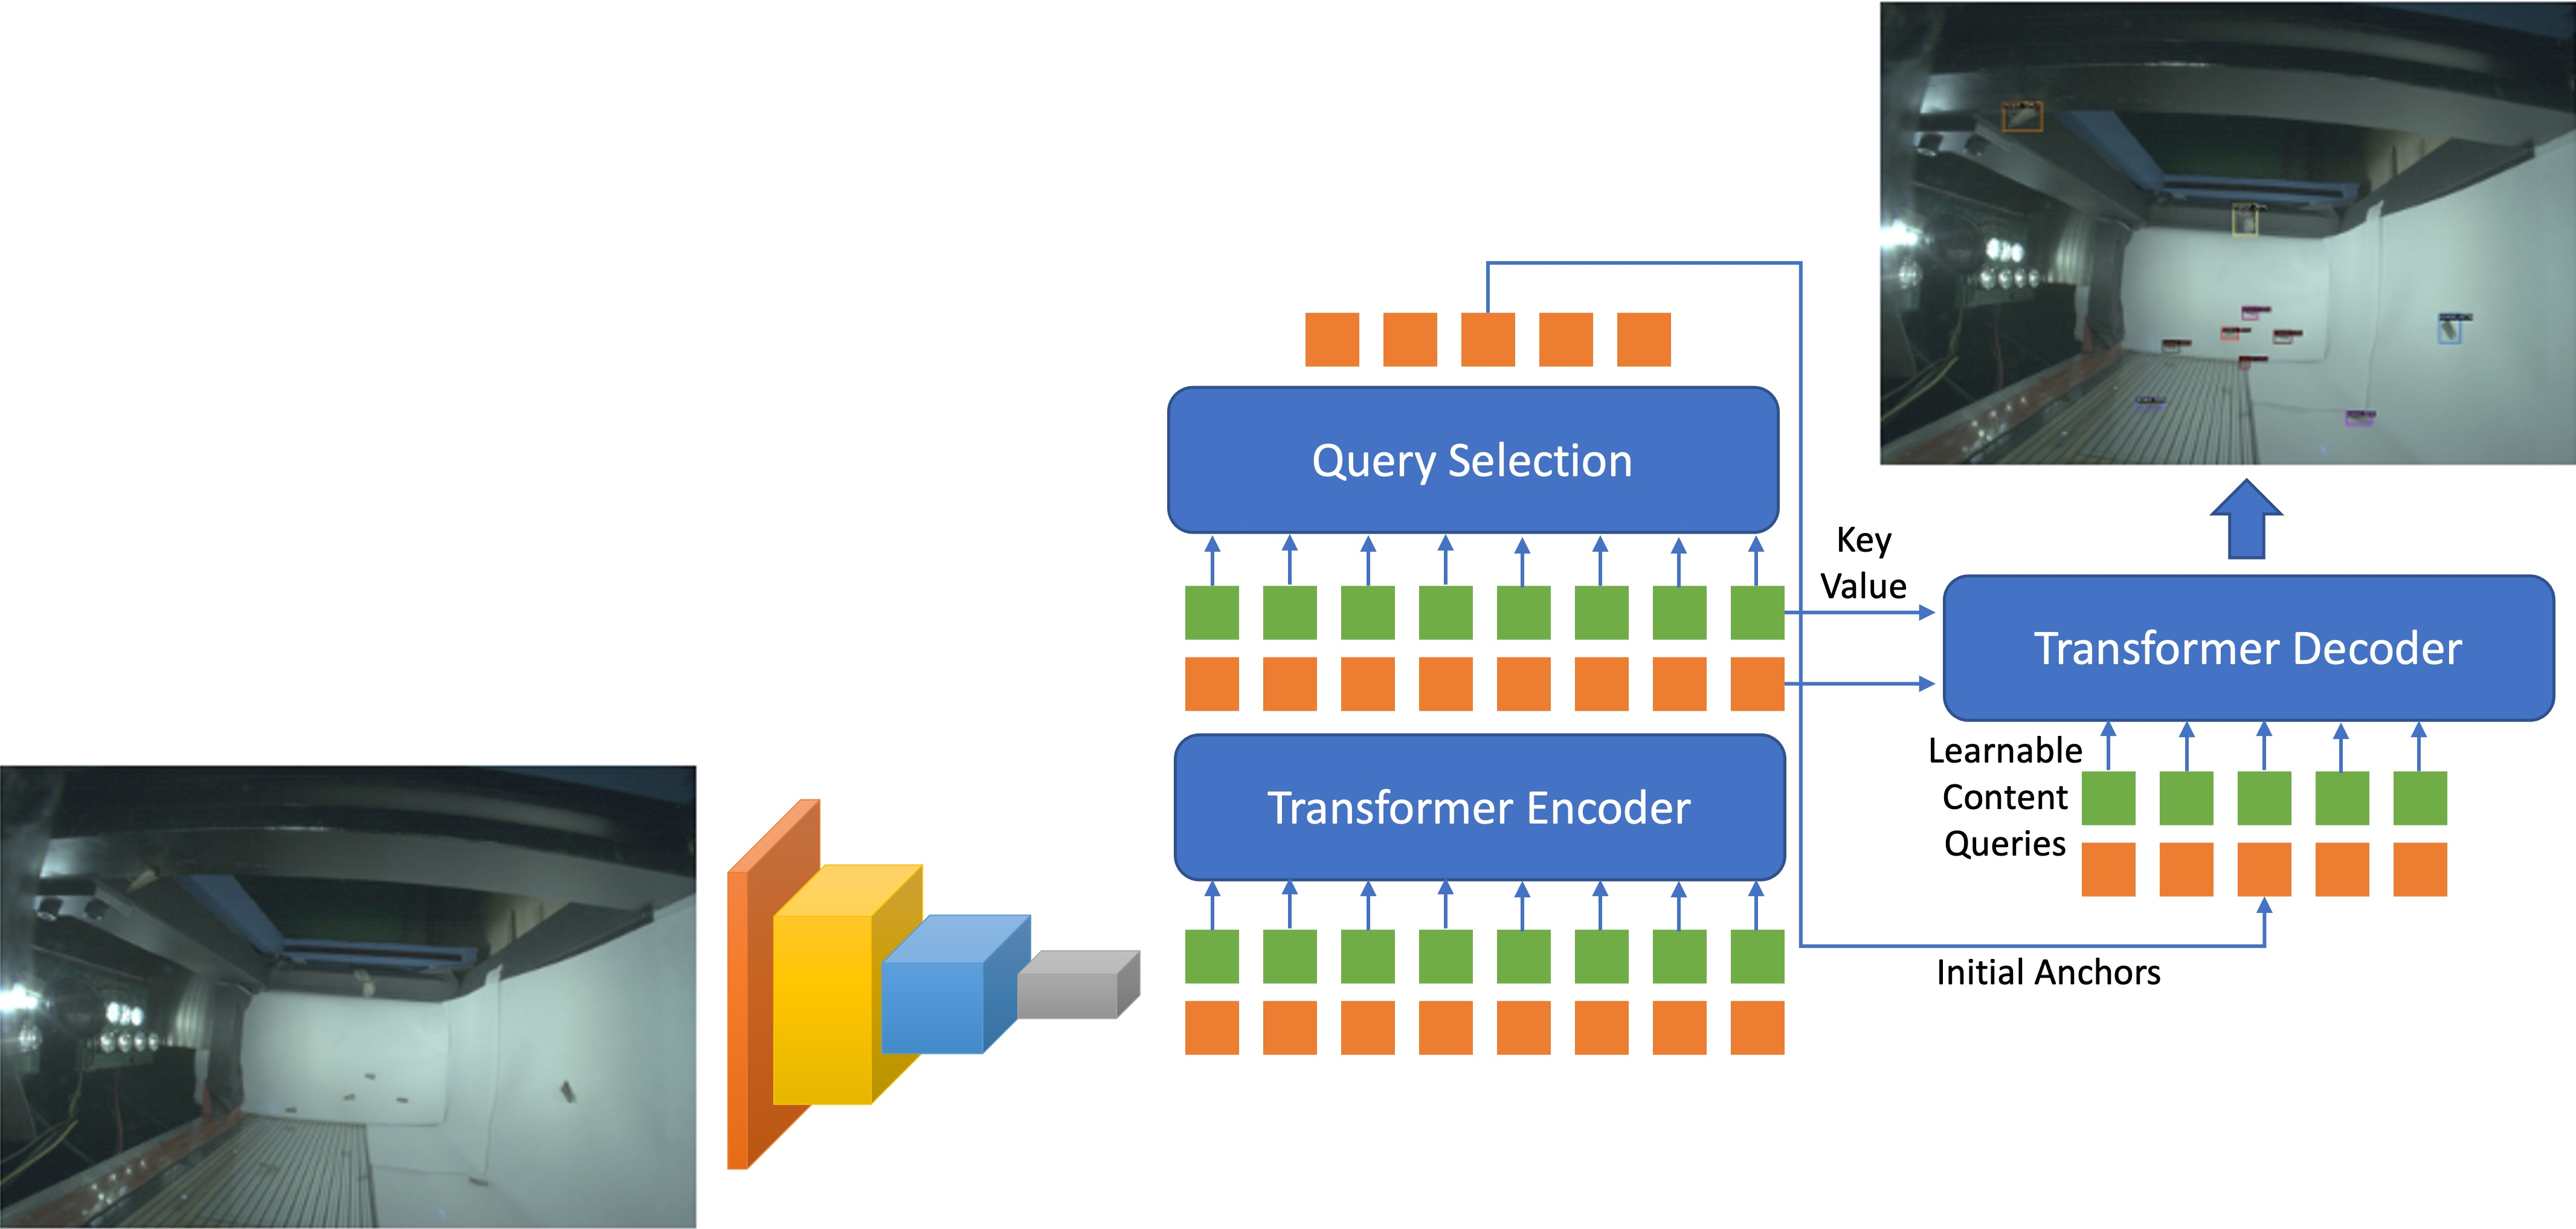
\includegraphics[width=1.0\linewidth]{Honors_Thesis/Figures/3.3.jpg}
\end{center}
\caption{Bug system transformer diagram.}
\label{fig:3.3}
\end{figure}

\section{Generative Pretrained Transformer (GPT)}
The Generative Pretrained Transformer (GPT) is a groundbreaking large language model (LLM) based on the Transformer architecture that leverages unsupervised learning for natural language understanding tasks. The underlying principle of GPT is a two-step process that involves unsupervised pre-training followed by supervised fine-tuning. Initially, the model is trained on a large unannotated text corpus to learn a general language representation. Subsequently, it is fine-tuned on specific, smaller labeled datasets for targeted tasks \cite{radford_narasimhan_salimans_sutskever}.

The GPT model employs a variety of masked language modeling called ``masked multi-head self-attention," which allows it to scale to longer sequences and capture long-range dependencies more effectively than traditional recurrent neural networks (RNNs). The Transformer architecture at the core of GPT enables the model to process input tokens in parallel, resulting in improved computational efficiency and scalability compared to RNNs and LSTMs.

A key aspect of GPT's success is its ability to achieve state-of-the-art performance across various natural language understanding tasks, including sentiment analysis, natural language inference, and question answering. By leveraging a generative language model for unsupervised pre-training and fine-tuning for specific tasks, GPT outperforms previous models by a significant margin \cite{radford_narasimhan_salimans_sutskever}.

As GPT has evolved through different versions, such as GPT-3.5 and GPT-4, it has experienced significant improvements in model size, architecture, parameters, and performance. Each new version incorporates advancements in training techniques, data sources, and architectural refinements that enhance language understanding capabilities. Fig \ref{fig:3.4} shows the enormous gap in the number of parameters between GPT-4 and previous models.

\begin{figure}[H]
\begin{center}
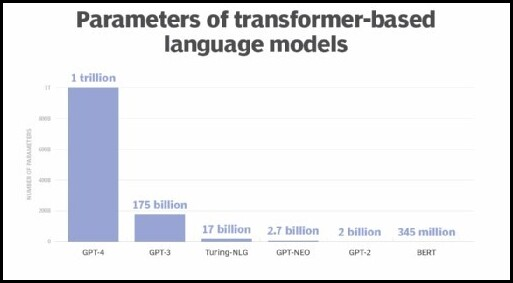
\includegraphics[width=0.8\linewidth]{Honors_Thesis/Figures/3.4.jpg}
\end{center}
\caption{Chart of No. of Parameters for multiple LLMs \cite{kerner_2023}.}
\label{fig:3.4}
\end{figure}

\subsection{Prompt Engineering}
Prompt engineering is the development and refinement of input prompts to guide the behavior of language models. It involves crafting the input text to effectively communicate the desired task to the model and elicit the desired response. Prompt engineering is important because the quality of the prompt can significantly impact the model's performance.

The choice of examples, the phrasing of the task, and other elements of the prompt can influence the model's understanding and output. For instance, in few-shot learning, the prompt may include a few examples of the task to be performed, followed by the specific instance on which the model should generate a response. Prompt engineering is still an active area of research, with development being done to create more effective prompts and evaluate model performance in various tasks for comparison \cite{prompt_eng_1, liu-etal-2021-noisy}.